% -*- mode: fundamental -*-

% Slides accompanying "Learn RISC-V CPU Implementation and BSV" book
% Copyright (c) 2024 Rishiyur S. Nikhil, All Rights Reserved

% -*- mode: fundamental -*-

% Slides accompanying "Learn RISC-V CPU Implementation and BSV" book
% Copyright (c) 2024 Rishiyur S. Nikhil, All Rights Reserved

% This is a preamble shared by all the slide decks

\documentclass[10pt, aspectratio=169]{beamer}

% \documentclass[17pt]{beamer}

% Avail. font sizes: 8pt, 9pt, 10pt, 11pt, 12pt, 14pt, 17pt, 20pt.
% Default font size is 11pt (= 22pt in full screen mode).

\usepackage{verbatim}
\usepackage{fancyvrb}
\usepackage{listings}

% ================================================================
% Themes

\usetheme{Madrid}          % Line at bottom: Author (affiliation), OptTitle, Conf, page 

% \usetheme{Copenhagen}    % Same as Madrid except bottom line: Author, OptTitle

% \usetheme{Berkeley}    % Takes up 1-inch border on left and top

% ----------------
% colorthemes
% (default), beaver, beetle, seahorse, wolverine

\usecolortheme{seahorse}

% ================================================================
% Customization: show table of contents before each section
% Use \AtBeginSubsection    to show before each subsection

% \AtBeginSection[]
% {
%   \begin{frame}
%     \frametitle{Table of Contents}
%     \tableofcontents[currentsection]
%   \end{frame}
% }

% ================================================================

% ----------------
% The bsc compiler and BSV language
\newcommand{\bsc}{\emph{bsc}}
\newcommand{\BSV}{\bf{BSV}}
% ----------------
% ITALICISE WORDS
\newcommand{\ie}{\emph{i.e.,}}
\newcommand{\eg}{\emph{e.g.,}}
\newcommand{\Eg}{\emph{E.g.,}}
\newcommand{\etc}{\emph{etc.}}
\newcommand{\via}{\emph{via}}
\newcommand{\vs}{\emph{vs.}}

% ----------------
% EMPTY BOXES OF VARIOUS WIDTHS, FOR INDENTATION

\newcommand{\hm}{\hspace*{1em}}
\newcommand{\hmm}{\hspace*{2em}}
\newcommand{\hmmm}{\hspace*{3em}}
\newcommand{\hmmmm}{\hspace*{4em}}

% ----------------
% Convenient widths

\newlength{\hlessmm}
\setlength{\hlessmm}{\textwidth}
\addtolength{\hlessmm}{-2em}

\newlength{\hlessmmm}
\setlength{\hlessmmm}{\textwidth}
\addtolength{\hlessmmm}{-3em}

\newlength{\hlessmmmm}
\setlength{\hlessmmmm}{\textwidth}
\addtolength{\hlessmmmm}{-4em}

% ================================================================
% Title page

\title[Learn CPU design \& BSV]{Learn RISC-V CPU Implementation and BSV}

\subtitle{(BSV: a High-Level Hardware Design Language)}

\author[{\copyright} R.S.Nikhil]{Rishiyur S.~Nikhil}
% \institute{Bluespec, Inc.}

% Date is set differently in each slide deck

% \logo{
\includegraphics[height=0.6cm]{../Figures/Bluespec_Logo_2022-10}}

% End of preamble
% ****************************************************************


\date{L4: BSV: Combinational Circuits}

% ----------------
% Switch off "pause" during development

\renewcommand{\PAUSE}[1]{#1}
% \renewcommand{\PAUSE}[1]{#1\pause}

% ****************************************************************

\begin{document}

% ================================================================

\begin{frame}
 \titlepage

 \begin{center}
  
\includegraphics[height=1cm]{../Figures/Bluespec_Logo_2022-10}
 \end{center}

\end{frame}

% ================================================================

\begin{frame}
\frametitle{Two CPU implementations (microarchitectures): Drum and Fife}

\begin{center}
\frame{\includegraphics[width=0.8\textwidth]{../Figures/Fig_Two_Microarchitectures}}
\end{center}

\footnotesize

We start learning BSV by coding the {\tt fn\_XXX} functions.  \\
These are used in both Drum and Fife, and are all combinational circuits.

\vspace*{1ex}

We start with {\tt fn\_Decode}.

\end{frame}

% ================================================================

\begin{frame}
\frametitle{Inputs to {\tt fn\_Decode}}

\footnotesize

The inputs to the Decode stage (see diagram on previous slide) are:

\PAUSE{\vspace{1ex}}

\begin{itemize}

 \item (From IMem (``instruction-memory'')): A 32-bit piece of data---a
 RISC-V instruction---that has become available by reading it from
 memory at the PC address.\footnote{When
 implementing the so-called ``C'' RISC-V ISA extension (``compressed
 instructions''), instructions can also be 16-bits, but we
 ignore that for now.}

 \PAUSE{\vspace{4ex}}

 \item (Direct from Fetch stage): any additional information for this
     instruction that did not need to go to memory and back.

\end{itemize}

\PAUSE{\vspace{4ex}}

We will use a BSV ``{\tt struct}'' type (to be described soon)
whenever we carry multiple pieces of data together.

\vspace{1ex}

Example: a memory request will carry a request-code (such as READ) and
an address together.

\end{frame}

% ================================================================

\begin{frame}
\frametitle{Outputs from {\tt fn\_Decode}}

\footnotesize

The outputs from the Decode stage, as shown in the diagram are:

\PAUSE{\vspace{1ex}}

\begin{itemize}

 \item Was the Fetch itself successful, or did it encounter a memory
   error; if so, what kind of memory error?

 \PAUSE{\vspace{1ex}}

 \item Is it a legal 32-bit instruction?

 \PAUSE{\vspace{1ex}}

 \item If legal, what is its broad classification: Control (Branch or
   Jump)? Integer Arithmetic or Logic? Memory Access?  This will help
   in choosing the next stage to which we must dispatch to execute the
   instruction.

 \PAUSE{\vspace{1ex}}

 \item Does it have zero, one or two input registers (``rs1'' and
   ``rs2'')?  If so, which ones?  This will help the next stage in
   reading registers.

 \PAUSE{\vspace{1ex}}

 \item Does it have zero or one output registers (``rd'')?  If so,
   which one?  This will help the final Register Write stage in
   writing back a value to a register.

\end{itemize}

\PAUSE{\vspace{2ex}}

To compute these values, we will need to extract ``slices'' of the
32-bit instruction (opcode, funct3, rs1, rs2, rd, ...) and compare
them with binary constants.

\end{frame}

% ================================================================

\begin{frame}[fragile]
\frametitle{BSV: Integer literals (constants)}

\footnotesize

Integer literals use the same notation as in Verilog and SystemVerilog:

\vspace{1ex}

\begin{Verbatim}[frame=single, numbers=left]
3'b010            // Binary literal, 3 bits wide
7'b_110_0011      // Binary literal, 7 bits wide
5'h3              // Hex literal, 5 bits wide
32'h3             // Hex literal, 5 bits wide
32'h_efff_0f17    // Hex literal, 32 bits wide (an AUIPC instruction)
'h23              // Hex literal, context determines width
\end{Verbatim}

\PAUSE{\vspace{1ex}}

When the size is omitted, {\bsc} will infer the required size from the
context, and extend it if necessary (zero-extend if the context
requires a \verb|Bit#(n)|, sign-extend if \verb|Int#(n)|).

\end{frame}

% ================================================================

\begin{frame}[fragile]
\frametitle{BSV: Identifiers and comments}

\footnotesize

{\bf Identifiers:} same as in most programming languages: any sequence
of alphabets, digits, and ``\verb|_|'' (underscore) characters,
beginning with an alphabet.

\vspace{1ex}

The upper/lower case of the first letter (always an alphabet) is important:
\begin{itemize}
 \item Uppercase first letter: constants (value constants, type constants).

   Examples:
   \begin{itemize}\footnotesize
    \item Value constants: \verb|True|, \verb|False|, \verb|MEM_RSP_OK|, ...
    \item Type constants: \verb|Bit|, \verb|Int|, \verb|Tuple2|, \verb|Vector|, ...
   \end{itemize}

 \vspace{1ex}

 \item Lowercase first letter: variables (value variables, type variables).

       Examples: \verb|x|, \verb|y|, \verb|tmp|, \verb|pc|, \verb|rg_pc|, \verb|has_rs1|, ...

\end{itemize}

\PAUSE{\vspace{10ex}}

{\bf Comments:} same as in Verilog/SystemVerilog/C/C++:
\begin{itemize}
 \item ``\verb|//|'' introduces a comment until end-of-line

 \item ``\verb|/*|'' and ``\verb|*/|'' bracket an unlimited amount of
       comment text (can span multiple lines)
\end{itemize}

\end{frame}

% ================================================================

\begin{frame}[fragile]
\frametitle{BSV: Introduction to Types (Data Types)}

\footnotesize

\begin{center}
 \frame{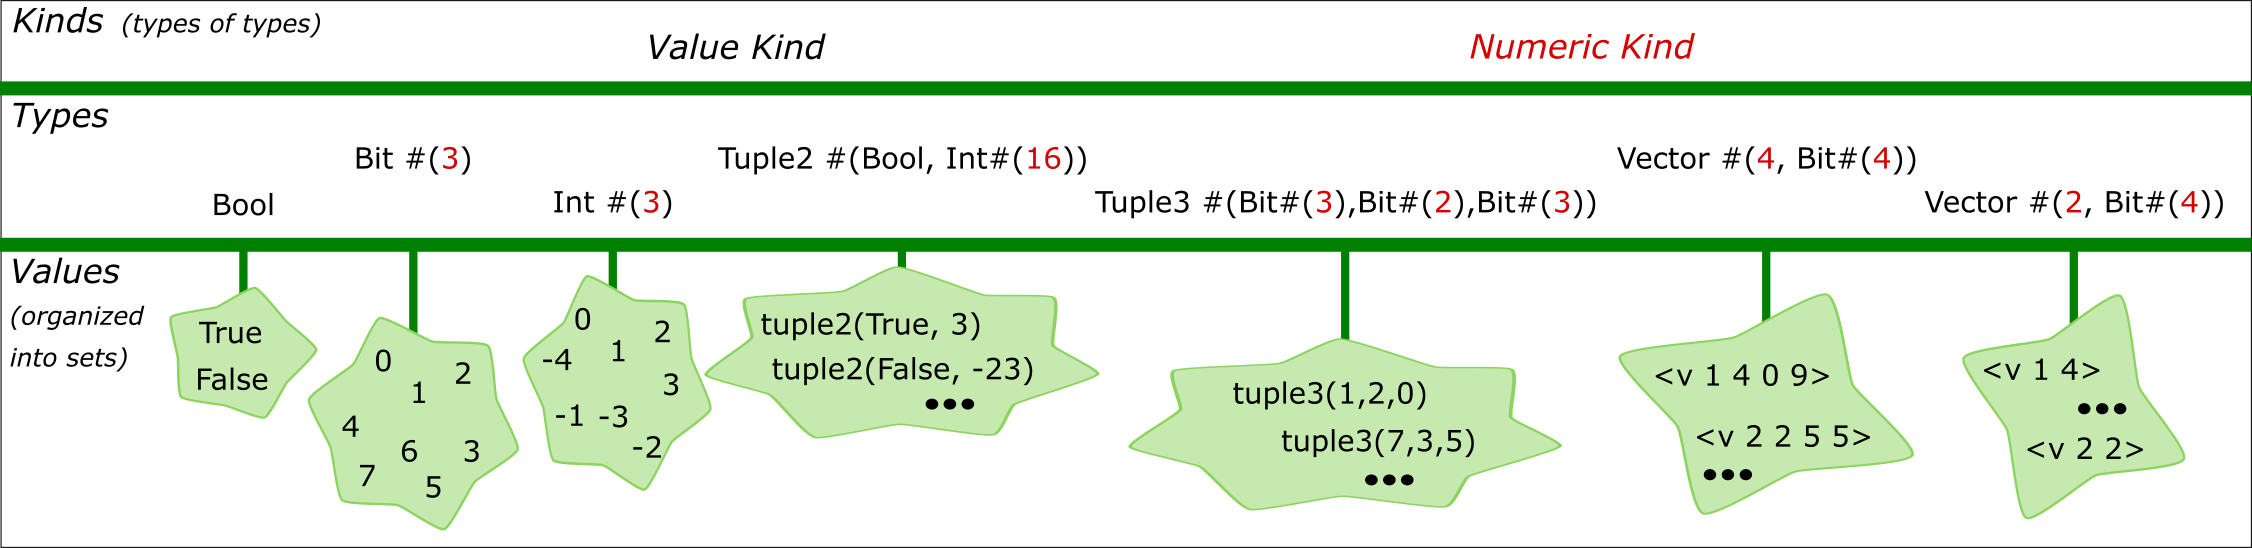
\includegraphics[width=\textwidth]{../Figures/Fig_BSV_Types}}
\end{center}

\vspace{1ex}

\begin{itemize}
 \item Programs (and hardware modules) compute with \emph{Values}.

 \item We group values into sets, which we call \emph{Types}.

 \item Types themselves have a ``type'' (\emph{Kind}):
       \begin{itemize}\footnotesize

        \item those representing actual values (\emph{Value Kind})

	\item those that describe some ``size'' feature of a type
              (\emph{Numeric Kind}, shown in red)

       \end{itemize}

\end{itemize}

Every operator, function and method declaration in BSV specifies the
types of its arguments and results, which is used by {\bsc} for strict
typechecking.

\end{frame}

% ================================================================

\begin{frame}[fragile]
\frametitle{BSV: Introduction to Types (Data Types)}

\footnotesize

Types can nested to arbitrary depth:

\begin{tabbing}
 \hmmmm \emph{type} ::= \emph{type-constructor} {\tt \#(} \emph{type}, ..., \emph{type} {\tt )}
\end{tabbing}

\vspace{2ex}

A \emph{type-constructor} always begins with an upper-case letter (is a type constant).

\vspace{2ex}

For each \emph{type-constructor}, each \emph{type} argument
(parameter) is fixed to be either of value kind or numeric kind.

For example,

\begin{itemize}

 \item In \verb|Bit #(n)|, \verb|n| is always of numeric kind.

 \item In \verb|Vector #(n,t)|, \verb|n| is always of numeric kind,
 \verb|t| is always of value kind.

 \item In \verb|Tuple3 #(t1,t2,t3)|, all three parameters are always of value kind.

\end{itemize}

\end{frame}

% ================================================================

\begin{frame}[fragile]
\frametitle{Bit-vectors in BSV}

\footnotesize

\begin{itemize}

 \item The basic type in any hardware design language is the
       bit-vector (a vector of $n$ bits) to be treated as a single
       entity.  Bit-vectors are carried on wires ($n$-bit vectors on
       $n$ wires), stored in registers, memories and other state
       elements.

 \vspace{1ex}

 \item The type of a bit-vector of $n$ bits in BSV is written: {\tt
       Bit\#($n$)}.

 \vspace{1ex}

 \item We can declare identifiers with a type just like in Verilog,
       SystemVerilog and C, with an initialization:

 \vspace{1ex}

 \begin{Verbatim}[frame=single, numbers=left]
   Bit #(32) pc_val = ?;
   Bit #(32) pc_val = 32'h_8000_0000;
   Bit #(32) pc_val = 'h_1000;
 \end{Verbatim}

 \vspace{1ex}

 Line 1: we let {\bsc} pick an initial value (usually picks
 \verb|'h_AAAA_..._AAAA| for visibility during debugging).

 \vspace{1ex}

 Line 2: the initial value is specified as an exactly 32-bit value,
 which matches the declared type of the identifier.

 \vspace{1ex}

 Line 3: the constant does not specify a width; {\bsc} will infer that
 it should be 32 bits, and will zero-extend the given 16 bits.

\end{itemize}

\end{frame}

% ================================================================

\begin{frame}[fragile]
\frametitle{Extracting smaller bit-vectors (``slicing''), or individual bits, from a bit-vector}

\footnotesize

\begin{Verbatim}[frame=single, numbers=left]
   Bit #(12) page_offset = pc_val [11:0];
   Bit #(1)  pc_lsb      = pc_val [0];
   Bit #(1)  pc_msb      = pc_val [31];
\end{Verbatim}

\vspace{1ex}

{\bsc} checks that the bit-widths match exactly and reports an error otherwise. \\
(there is no silent bit-extending or truncating).

\end{frame}

% ================================================================

\begin{frame}[fragile]
\frametitle{Operators for bit-vectors}

\footnotesize

Left- and right-arguments must have same \verb|Bit#(n)| type.

\vspace{1ex}

Comparison ops: result type is {\tt Bool}
\begin{Verbatim}[frame=single, numbers=left]
   if (a == b) ...;        // equality
   if (a != b) ...;        // not-equal to
   if (a < b) ...;         // less-than
   if (a <= b) ...;        // less-than-or-equal-to
   if (a > b) ...;         // greather-than
   if (a >= b) ...;        // greater-than-or-equal-to
\end{Verbatim}

Arithmetic ops: result type is same as argument types
\begin{Verbatim}[frame=single, numbers=left]
   x = a + b - c * d;      // add, subtract, multiply
\end{Verbatim}

Bitwise logic ops: result type is same as argument types:
\begin{Verbatim}[frame=single, numbers=left]
   //   AND  OR   unary INVERT   XOR  XNOR  XNOR
   x = a &  b |     (~ c)         ^   d ^~ e ~^ f;
\end{Verbatim}

Left- and Right-Shifts:
\begin{Verbatim}[frame=single, numbers=left]
   x = (a << 3) & (b >> 14);
\end{Verbatim}

\end{frame}

% ================================================================

\begin{frame}[fragile]
\frametitle{Integer types in BSV}

\footnotesize

\begin{Verbatim}[frame=single, numbers=left]
   Bit #(n)        // bit-vectors, bounded to n bits
   Int #(n)        // signed integers, bounded to n bits
   UInt #(n)       // unsigned integers, bounded to n bits
   Integer         // Mathematical integers (unbounded, no bit-width limit)
\end{Verbatim}

\vspace{2ex}

\begin{itemize}

 \item We rarely use \verb|UInt#(n)| because they are the same as
        \verb|Bit#(n)| (``isomorphic'').

 \item \verb|Integer| is used for values that are only meaningful at
     compile time and never represented in hardware (such as the size
     of a vector of interfaces or modules).

\end{itemize}

\end{frame}

% ================================================================

\begin{frame}[fragile]
\frametitle{Explicit extension and truncation}

\footnotesize

\begin{Verbatim}[frame=single]
   y = zeroExtend (x);
   y = signExtend (x);
   y = extend (x);
   x = truncate (y);
\end{Verbatim}

\vspace{2ex}

\begin{itemize}
 \item {\tt x} and {\tt y} must both be \verb|Bit#(..)| or both be \verb|Int#(..)|
 \item Bit-width of {\tt y} must be $\geq$ Bit-width of {\tt x}
 \item \verb|extend| will zero-extend for \verb|Bit#(..)| and sign-extend for \verb|Int#(..)|
\end{itemize}

\end{frame}

% ================================================================

% % -*- mode: fundamental -*-

% Slides accompanying "Learn RISC-V CPU Implementation and BSV" book
% Copyright (c) 2024 Rishiyur S. Nikhil, All Rights Reserved

% This is a postamble shared by all the slide decks

% ================================================================

\begin{frame}

\begin{center}
  {\LARGE End}
\end{center}

\end{frame}

% ================================================================


% ****************************************************************

\end{document}


\vspace{1ex}

{\bsc} will not truncate a too-large constant; instead it will give an
error message.
